%\documentclass[letterpaper, 10 pt, conference]{ieeeconf}  
\documentclass[a4paper, 10pt, conference]{ieeeconf}      

\IEEEoverridecommandlockouts                             
\overrideIEEEmargins

\usepackage[T1]{fontenc}
\usepackage{amsmath}
\usepackage{amsfonts}
\usepackage{amssymb}
\DeclareMathOperator*{\argmax}{argmax}
\usepackage{tabularx}
\usepackage{graphicx}
\usepackage{algorithm}
%\usepackage{algorithmic}
\usepackage{algpseudocode}
\usepackage{mathtools}

\DeclarePairedDelimiter\abs{\lvert}{\rvert}%

\title{\LARGE \bf
Scalable Low latency Live SVC Video Streaming using SDN
}

\author{Eyal Azran$^{1}$ and Dr. Amit Dvir$^{2}$% <-this % stops a space
\thanks{$^{2}$Dr. Ofir Pele
        {\tt\small }}%
}

\begin{document}

\maketitle
\thispagestyle{plain}
\pagestyle{empty}

\begin{abstract}

%We address the challenge of optimizing the delivery of high quality low latency live video streaming over Software Defined Network (SDN) enabled routers. Specifically, we consider real-time Scalable Video Coding (SVC) streaming where clients can join and leave the streaming services dynamically. SDN decouples network control and management from data forwarding and enable us to leverage the OpenFlow-controlled network orchestration for efficient  streaming to heterogeneous clients. SVC
%is capable of bit stream adaptation by applying a layered approach. We route each video layer over a different multicast distribution tree while optimizing a cost function that consider the subscriber priority, delay from source, link utilization, etc. The problem of constrained shortest path is known a NP-Complete, so we propose a heuristic algorithm and compare it to current practices. Results show our approach can achieve effective performance improvements in terms of video Quality of Experience (QoE) and network resource utilization.

Software Define Networks (SDN)s decouples network control and management from data forwarding and enables leverage the OpenFlow-controlled network orchestration for efficient real time S... V.... C... (SVC) video streaming. 

 One of the main challenges is how to optimize the delivery of high quality low latency live video streaming over SDN enabled routers.
 
 Specifically, we consider real-time Scalable Video Coding (SVC) streaming where clients can join and leave the streaming services dynamically. In this problem, we should route each video layer over a different multicast distribution tree while optimizing a cost function that consider the subscriber priority, delay from source, link utilization, etc. 
 
 Therefore, the problem is similar to constrained shortest path which is known a NP-Complete. We propose a heuristic algorithm and compare it to current practices. 
 
 Results show our approach can achieve effective performance improvements in terms of video Quality of Experience (QoE) and network resource utilization

\end{abstract}

\begin{keywords}
Software Defined Network, Scalable Video Coding, Multicast, Live Streaming, Heterogeneous Clients
\end{keywords}


\section{INTRODUCTION}

\subsection{Software Defined Network (SDN)}

\subsection{Scalable Video Coding (SVC)}

\section{Related Work}

\section{Contribution of Our Work}

\section{System Design}
Video Manager - two-way communication with subscribers and video sources. capability of the subscribers for suitable video layers. Admission control. Billing. heartbeat mechanism to determine whether the subscriber is still connected. The subscriber is responsible to initiate the I'm alive messages periodically.

Video Sources - supports SVC encoding and
decoding, two-way communication with Video Manager
different layers of the video are transmitted
at different user datagram protocol (UDP)
source ports

Video SUbscribers - supports SVC encoding and
decoding, two-way communication with Video Manager. can be
smartphones, tablets, notebooks, HDTVs, and so on
different terminals
can subscribe to different suitable video layers

SDN Controller - two-way communication with network elements 
high-level routing decisions
build multiple
multicast trees for the same video of different
layers
LLDP
detect congestion
reconfigure network to handle congestion

uses ‘statistics’ messages to detect the congestion event
out-of band control network with network elements

OpenFlow Enabled Network Elements, two-way communication with SDN controller

\section{PROBLEM FORMULATION}

\newcommand{\si}[1]{S_#1}
\newcommand{\lcsi}[1]{s_#1}
\newcommand{\lcli}[1]{l_#1}
\newcommand{\sil}[2]{S_{#1,#2}}
\newcommand{\lcsil}[2]{s_{#1,#2}}
\newcommand{\ri}[1]{R_#1}
\newcommand{\lcri}[1]{r_#1}
\newcommand{\vil}[3]{V(#1, #2, #3)}
\newcommand{\filj}[2]{F(#1, #2)}
\newcommand{\vri}[5]{V(#1, #2, #3, #4, #5)}
\newcommand{\numOfSrc}{N}
\newcommand{\numOfRcv}{M}
\newcommand{\lsi}[1]{L(#1)}
\newcommand{\tsil}[2]{T_{#1,#2}}
\newcommand{\tsilu}[3]{\tsil{#1}{#2}^{#3}}
\newcommand{\rsil}[1]{R(#1)}
\newcommand{\ptsiluv}[3]{P(#1,#2, #3)}
\newcommand{\psilj}[3]{P_{#1,#2,#3}}
\newcommand{\delay}[1]{d(#1)}
\newcommand{\bsil}[1]{b(#1)}
\newcommand{\dsil}[1]{d(#1)}
\newcommand{\jsil}[1]{\sigma(#1)}
\newcommand{\psil}[1]{p(#1)}
\newcommand{\buv}[2]{b(#1,#2)}
\newcommand{\duv}[2]{d(#1,#2)}
\newcommand{\juv}[2]{\sigma(#1,#2)}
\newcommand{\puv}[2]{p(#1,#2)}
\newcommand{\w}[1]{w_{#1}}
\newcommand{\ci}[1]{c_{#1}}
\newcommand{\g}[1]{G(#1)}
\newcommand{\contentMaxDelay}[1]{\delta_{#1}}
\newcommand{\contentMaxJitter}[1]{\sigma_{#1}}
\newcommand{\pri}[1]{P_{\ri{#1}}}
%\newcommand{\maxLayerri}[1]{L_{\ri{#1}}^max}

% New definitions
\algnewcommand\algorithmicswitch{\textbf{switch}}
\algnewcommand\algorithmiccase{\textbf{case}}
\algnewcommand\algorithmicassert{\texttt{assert}}
\algnewcommand\Assert[1]{\State \algorithmicassert(#1)}%
% New "environments"
\algdef{SE}[SWITCH]{Switch}{EndSwitch}[1]{\algorithmicswitch\ #1\ \algorithmicdo}{\algorithmicend\ \algorithmicswitch}%
\algdef{SE}[CASE]{Case}{EndCase}[1]{\algorithmiccase\ #1}{\algorithmicend\ \algorithmiccase}%
\algtext*{EndSwitch}%
\algtext*{EndCase}%


Consider a network that is represented by a directed graph,
G= (V, E), where V is the set of vertices and E is the set of edges.
Video servers (Sources) and clients (recievers) are represented as graph's vertices.
One server may serve multiple contents, each is represented as graph's vertex. Each edge (u,v) has multiple weights - Delay $\duv{u}{v}$, BW b(u,v) and probability of packet loss p(u,v). The wehights of each link (u,v) are not necessairly symetric, ie: 
\[d(u,v) \neq d(v,u)\] 
\[b(u,v) \neq b(v,u)\]
\[p(u,v) \neq p(v,u)\]

\begin{table}[ht]
\caption{Basic symbols and acronyms} 
\begin{center}
\label{tab:LISTOFABBREVIATIONS1}
\begin{tabular}{|p{1cm}|p{6cm}|}
\hline
    \textbf{Symbol} & \textbf{Description} \\
    $bps$   & Bit per second \\\hline
    $ms$    & Miliseconds \\\hline
    $G$     & Graph representing the network  \\\hline
    $V$    	&  Graph's vertices set, the network routers, sources and recievers
     \\\hline
    $E$ 	& Graph's edges set, the network links \\\hline
    \text{SVC}	& Scalebale Video Coding \\\hline	
\end{tabular}
\end{center}
\end{table}

\begin{table}[ht]
\caption{Problem formulation and algorithm's symbols - Cont} 
\begin{center}
\label{tab:LISTOFABBREVIATIONS2}
\begin{tabular}{|p{1cm}|p{6cm}|}
\hline
    \textbf{Symbol} & \textbf{Description} \\
    \hline
		$\si{i}$ & A video source, represented by a graph's vertex \\\hline
		$\sil{i}{l}$ & Layer $l$ of source $\si{i}$ \\\hline
		$\ri{i}$ & A video reciever, represented by a graph's vertex \\\hline
		$\numOfSrc$ & Number of sources \\\hline
		$\numOfRcv$ & Number of recievers \\\hline
		$\lsi{\si{i}}$ & Number of layers of source $S_i$ \\\hline
		$\tsil{\si{i}}{l}$ & Sub graph of G, generated for the $l^{th}$ layer of source $S_i$ \\\hline
		$\rsil{\sil{i}{l}}$	& The set of recievers who requested the $l^{th}$ layer of source $\si{i}$ \\\hline
		$\psilj{i}{j}{l}$ & The path from $\si{i}$ to $\ri{j}$ in $T({S_{i,l}})$ \\\hline		
		$\bsil{\sil{i}{l}}$ & Minimum bandwidth for the $l^{th}$ layer of source $\si{i}$ \\\hline
		$\buv{u}{v}$ & The bandwidth [bps] of edge \\\hline
		$\duv{u}{v}$ & The delay [ms] of a packet traversing from u to v \\\hline
		$\dsil{\psilj{i}{j}{l}}$ & Delay of the path from $\si{i}$ to $\ri{j}$ in $T({S_{i,l}})$ \\\hline
		$\juv{u}{v}$ & Jitter [ms] from u to v. The jitter is the std of d(u,v) \\\hline
		$\jsil{\psilj{i}{j}{l}}$ & Jitter of the path from $\si{i}$ to $\ri{j}$ in $T({S_{i,l}})$ \\\hline
		$\puv{u}{v}$ & Probability of packet traversing edge u to v to get dropped \\\hline	
		$\psil{\psilj{i}{j}{l}}$ & Packet loss of the path from $\si{i}$ to $\ri{j}$ in $T({S_{i,l}})$ \\\hline
		$\contentMaxDelay{i}$ & Max delay allowed for contect $i$ \\\hline
		$\contentMaxJitter{i}$ & Max jitter allowed for contect $i$ \\\hline
\end{tabular}
\end{center}
\end{table}


\begin{table}[ht]
\caption{Problem formulation and algorithm's symbols - Cont} 
\begin{center}
\label{tab:LISTOFABBREVIATIONS3}
\begin{tabular}{|p{5cm}|p{2cm}|}
\hline
    \textbf{Symbol} & \textbf{Description} \\\hline
    $\vri{\ri{j}}{\sil{i}{l}}{\dsil{\psilj{i}{j}{l}}}{\jsil{\psilj{i}{j}{l}}}{\psil{\psilj{i}{j}{l}}}$ & The reciever's value to the company based on Quality of Delivery (QoD) parameters
     \\\hline
\end{tabular}
\end{center}
\end{table}

Definitions:
\newline

% delay
Path's Delay:
\begin{equation}
\dsil{\psilj{i}{j}{l}}= \sum_{(u,v) \in P_{i,j,l} } \duv{u}{v}
\end{equation}

% jitter
Path's Jitter:
\begin{equation}
\jsil{\psilj{i}{j}{l}} = \sum_{ (u,v) \in P_{i,j,l} } \juv{u}{v}
\end{equation}

% error rate
Path's probability of loss:
\begin{equation}
\psil{\psilj{i}{j}{l}} = 1 - (\prod_{(u,v) \in P_{i,j,l}}(1 - \puv{u}{v}))
\end{equation}

For every $t \geq 0$ time units that layer $l$ of content $i$ is streamed, the revenue for the company is:
% V
\begin{equation}
\vil{i}{l}{t} = t \cdot \sum_{\ri{j} \in \tsil{\sil{i}{l}}{}} \g{i} \cdot \filj{l}{j}
\end{equation}

% G
\begin{equation}
\g{i} = \begin{cases}
\ci{1} 	&\quad type(\si{i}) = Critical  	\\
\ci{2} 	&\quad type(\si{i}) = Regular  		\\
\ci{3} 	&\quad type(\si{i}) = Low   		\\
0 		&\quad\text{otherwise.} 			\\ 
\end{cases}
\end{equation}

% F
\begin{equation}
\filj{l}{j} = 
\begin{cases}
    \w{1} 	&\quad \pri{j} = GOLD \quad , l = BL \\
    \w{2} 	&\quad \pri{j} = SLVR \quad , l = BL \\
    \w{3} 	&\quad \pri{j} = GOLD \quad , l = EL \\
    \w{4} 	&\quad \pri{j} = BRNZ \quad , l = BL \\
    \w{5} 	&\quad \pri{j} = SLVR \quad , l = EL \\
    \w{6} 	&\quad \pri{j} = BRNZ \quad , l = EL \\
    0 		&\quad\text{otherwise} \\ 
\end{cases}
\end{equation}

where:
% w1 < w2 < ... 
\begin{equation}
\w{1} \ge \w{2} \ge \w{3} \ge \w{4} \ge \w{5} \ge \w{6} \ge \w{7}
\end{equation}

Our goal is:
\begin{equation}
\argmax_{T_{i=1,l=1}^{\numOfSrc , \lsi{\si{i}}} }{\sum_i \sum_l } vil{i}{l}{t} \quad , \quad 0 \le t \le T
\end{equation}

subject to:
\vspace{5mm} \newline
bandwidth constraint:
\begin{equation}
\min_{ (u,v) \in \tsil{i}{i} \buv{u}{v} \ge \bsil{\sil{i}{l}}} \quad \forall i \ge 0, \quad \forall l \ge 1
\end{equation}

Delay constraint
\begin{equation}
\dsil{\psilj{i}{j}{l}} \le \contentMaxDelay{i} \quad \forall i %\ge 0, \quad \forall l \ge 0, \quad \forall \ri{j} \in \tsil{\sil{i}{l}}
\end{equation}

Jitter constraint
\begin{equation}
\big(\jsil{\psilj{i}{j}{l}} \le \contentMaxJitter{i} \quad %\forall i \ge 0, \quad \forall l \ge 0, \quad \forall \ri{j} %\in \tsil{\sil{i}{l}})\big
\end{equation}

Video decodable Constraints:
\vspace{5mm} \newline
Once layer $l$ received, layer $l-1$ must be received:
\begin{equation}
\ri{j} \in \tsil{\sil{i}{l}} \Rightarrow \ri{j} \in \tsil{\sil{i}{l-1}} \quad \forall i \ge 0, \quad \forall l \ge 1
\end{equation}

Delay offset of layers $l$ and $l-1$ is no more than predefined value
\begin{equation}
\lvert \dsil{\psilj{i}{j}{l}} - \dsil{\psilj{i}{j}{l-1}} \rvert %\le T_{decodable} \quad \forall i \ge 0, \quad \forall l \ge 1, \quad \forall \ri{j} \in \tsil{\sil{i}{l}}
\end{equation}


\section{HEURISTIC ALGORITHMS}
\subsection{Low Latency Video Streaming (LLVS)}

Each requested layer of the same content is considered unique request.

\newpage

\begin{algorithm}
    \caption{LLVS}\label{alg:main}
    \begin{algorithmic}[1]
    \Procedure{main}{}
        \State $G \gets networkTopology()$
        \State $G_{(u,v)}^{\Gamma} \gets \emptyset$
        \State $G_{(u,v)}^T \gets \emptyset$
        \State $\Gamma \gets \emptyset$
        \State $T \gets \emptyset$
        \State $totalRevenue \gets 0$
        \While{$true$}
            \State $Event \gets waitForEvent()$
            \State $dynamicOperation(Event)$    
            \State $totalRevenue \gets totalRevenue+revenue()$
        \EndWhile
    \EndProcedure
    \end{algorithmic}
\end{algorithm}

\begin{algorithm}
    \caption{dynamicOperation}\label{alg:dynamicOperation}
    \begin{algorithmic}[1]
    \Procedure{dynamicOperation}{$Event$}
        \Switch{$Event$}
            \Case{$Event = requestAdded$}
                \State $addRequest()$
            \EndCase
            \Case{$Event = requestRemoved$}
                \State $removeRequest()$
            \EndCase
            \Case{$Event = linkFailed$}
                \State $linkFailure()$
            \EndCase
            \Case{$Event = nodeFailed$}
                \State $nodeFailure()$
            \EndCase
            \Case{$Event = sourceAdded$}
                \State $addSource()$
            \EndCase
            \Case{$Event = sourceRemoved$}
                \State $removeSource()$
            \EndCase
        \EndSwitch
    \EndProcedure
    \end{algorithmic}
\end{algorithm}
\begin{algorithm}
    \caption{addRequest}\label{alg:addRequest}
    \begin{algorithmic}[1]
    \Procedure{addRequest}{$\gamma$}
        \State $\tsil{\lcsi{i}}{\lcli{j}}$
    \EndProcedure
\end{algorithmic}
\end{algorithm}

\begin{algorithm}
    \caption{linkFailure}\label{alg:linkFailure}
    \begin{algorithmic}[1]
    \Procedure{linkFailure}{$(u,v)$}
        % \State $\Gamma' \gets \Gamma_{(u,v)}$
        \For{$\gamma \in \Gamma_{(u,v)}$}
            \State $\lcsi{k}\gets\gamma.source$ 
            \State $\lcli{k}\gets\gamma.layer$
            \State $removeUpperLayers()$
            \State $\tsil{\lcsi{k}}{\lcli{k}} = \tsil{\lcsi{k}}{\lcli{k}} / (u,v)$ \Comment{need to find affected clients}
            \State $\Gamma_{(u,v)} = \Gamma_{(u,v)} / (u,v)$
        \EndFor
    \EndProcedure
    \end{algorithmic}
\end{algorithm}

\begin{algorithm}
    \caption{nodeFailure}\label{alg:nodeFailure}
    \begin{algorithmic}[1]
    \Procedure{nodeFailure}{$u$}
    \EndProcedure
    \end{algorithmic}
\end{algorithm}

\begin{algorithm}
    \caption{revenue}\label{alg:revenue}
    \begin{algorithmic}[1]
    \Procedure{revenue}{}
    \EndProcedure
    \end{algorithmic}
\end{algorithm}

\begin{algorithm}
    \caption{handleRequest}\label{alg:handleRequest}
    \begin{algorithmic}[1]
    \Procedure{HandleRequest}{$G$,$\Gamma$}
        \State $\Gamma \gets sortByUserPriority(\Gamma)$
        \State $\Gamma \gets secondarySortByLayer(\Gamma)$
        \For{\texttt{$\gamma_k \in \Gamma$}} 
            \If{$\gamma_i.valid$ $=$ FALSE} 
            Break; 
            \EndIf
            \State $\lcsi{k}\gets\gamma_i.source$ 
            \State $\lcli{k}\gets\gamma_i.layer$ 
            \For{ $(u,v) \in \tsil{\lcsi{k}}{\lcli{k}}$ } 
                \State $\buv{u}{v} = \buv{u}{v} + \bsil{\lcsil{k}{\lcli{k}}}$
            \EndFor
            \State $G' \gets \emptyset$
            \For{ $(u,v) \in G$}
                \If{$\buv{u}{v} \ge \bsil{\lcsil{k}{\lcli{k}}}$}
                    \State $G' \gets (u,v) $
                \EndIf
            \EndFor
            \State $\psilj{\lcri{k}}{\lcsi{k}}{\lcli{k}} = shortestPathByLatency(\lcri{k} ,\lcsi{k})$
            \If{$\delay{\psilj{\lcri{k}}{\lcsi{k}}{\lcli{k}}} \ge \gamma_k.maxDelay$} Break; \EndIf
            \If{$\lcli{k} \ge 1$} \Comment{layer is not BASE}
                \If{$\abs{ \delay{\tsilu{\lcsi{k}}{\lcli{k}-1}{\lcri{k}}} - \delay{\psilj{\lcri{k}}{\lcsi{k}}{\lcli{k}}}} \ge \si{k}.mdd$} 
                \State Break; 
                \EndIf
            \EndIf
            \State $findIntersectionWithTree()$
            \State $addPathToNetwork();$
        \EndFor
    \EndProcedure
    \end{algorithmic}
\end{algorithm}

\subsection{Dynamic Operation of LLVS}
\subsection{Complexity Analysis}

\section{PERFORMANCE EVALUATIONS}

\subsection{Comparison with LBSLS}
\subsection{}

\section{Conclusion}

\newpage
\begin{figure}[htbp]
\centering
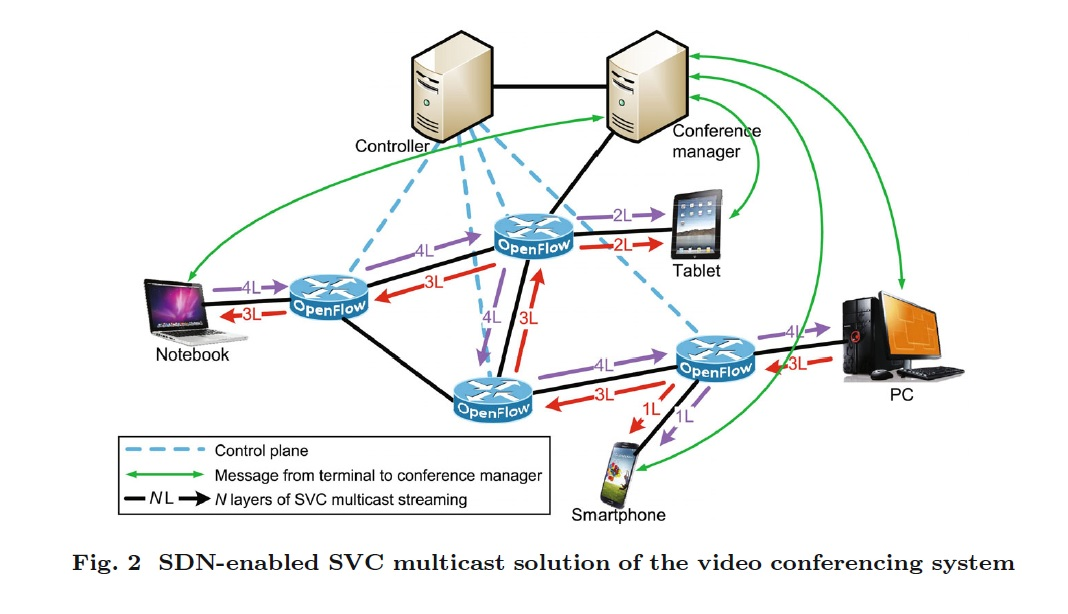
\includegraphics[scale=0.45]{svc-sdn-video-conf.jpg}
\caption{svc caption}
\label{svc label}
\end{figure}

\addtolength{\textheight}{-12cm}

\bibliographystyle{plain}
\bibliography{bibliography.bib}

\section{other papers}
to the desired quality of delivery defined by a set of constraints (minimum
packet loss / delay / jitter / overall bandwidth utilization). We propose
a graph based network model and formulate a constarint shortest path
problem which is known to be NP-Complete. Next, we design sacalable
and efficient heuristic, and compare the results to current practices. Results
show siginificant improvements in video quality and runtime of the
algorithm.


Software-Defined Networking
Multicast Video Streaming - 
Layered Content – Scalable Video Coding and Layered Path Routing
Differential QoS – BE, Assured Forwarding
Large Scale - Network, Content Providers, Subscribers
High Dynamicity – Subscribers join and leave dynamically and change their content requests
Subscriber priorities – Free, Regular, VIP
Global Maximum for company revenue
Self-Healing – Change path routing when network change occurs
Background traffic – simulate (as much as possible) real world scenario
OpenFlow - 
Intra and Inter domain - 

**** \cite{yang2014multicast} ****

In video streaming service, multicast mode is a
promising way to complement unicast delivery of content, since
it deliveries the video content to a broad range of receivers. It is
considered as an efficient scheme to reduce redundant traffic in
the networks. In this paper, we propose an OpenFlow based
architecture for implementing Scalable Video Coding (SVC)
multicast streaming. It enables in-network identifying, processing
and manipulating the media streams, which makes prompt
bitrate adaptation possible in response to network fluctuations.
The heterogeneous video quality demand from the heterogeneous
device also can be satisfied by customizing the multicast traffic
through a centralized OpenFlow controller. We implement a
testbed following the proposed architecture in our campus.
With OpenFlow, we deploy IP multicast in a new way without
Internet Group Management Protocol (IGMP) or any multicast
addresses. Experiments implemented on the testbed show that
our approach can provide a flexible and controllable video
multicast streaming service and improve the usage of bandwidth
resource in the condition of guaranteeing multicast receivers’
Quality of Experience (QoE).

reduce redundant traffic in the networks

we propose an OpenFlow based architecture for implementing Scalable Video Coding (SVC) multicast streaming

response to network fluctuations

our approach can provide a flexible and controllable video multicast streaming service and improve the usage of bandwidth resource in the condition of guaranteeing multicast receivers Quality of Experience (QoE)

Video traffic such as IPTV will account for 73 \% of total IP traffic by 2017. Most of the video applications that currently exist are implemented using unicast

Scalable Video Coding (SVC) \cite{schwarz2007overview} provides bit-stream scalability for graceful degradation transmission or adaptation, thus fulfilling the customized requirements like adapting to the heterogenous device capabilities and heterogeneous networks

For instance, when receivers are suffering from the network congestion, they can subscribe less layers from the layered SVC video source in order to avoid the annoying playback interruptions. 

Software-Defined Networking (SDN) \cite{sezer2013we} has been fast emerging as a promising network technology for building next-generation services and networks \cite{yang2014multicast}

makes it possible to implement multicast authentication, authorization, and accounting (AAA) integration for user authentication purpose in a multicast context

Related Work
SDN is a hot topic in the area of networks and very
attractive for the academia and industry. There have been
some works about SVC over OpenFlow networks. Civanlar et
al. [6] described an architecture for supporting QoS flows in
OpenFlow environment. Egilmez et al. [7] presented a solution
for optimizing forwarding decisions at the control layer to
enable dynamic QoS supporting, which extended the work [6].
However, they focused on the scenario of SVC transmission
using unicast. Multicast in OpenFlow network was widely considered
in the literature. Marcondes et al. proposed CastFlow
[8] aiming to reduce the multicast event delays. A design of
an OpenFlow controller handling IP multicast with Fast Tree
Switching in order to reduce packet loss has been investigated
in [9]. These works mainly discussed multicast issue, instead
of combining the SVC feature with multicast over OpenFlow
Networks.
SVC transmission with multicast can be categorized as
a layered multicast issue. Receiver-driven Layered Multicast
(RLM) was first introduced by Steven McCanne et al. [10]
for the transmission of layered signals over heterogeneous
networks using receiver-driven adaptation. Zhang et al. proposed
a receiver-driven router-assisted layered multicast protocol
(RALM) [11] which was based on the receiver-driven
layered approach and used router support to achieve enhanced
performance.

SVC is the scalable extension of H.264/AVC video coding
standard which encodes the signal once at highest resolution,
but enables decoding from partial streams depending on the
specific rate and resolution required by a certain application
[13].

However, in order to compromise with IP
protocol, the default destination IP/port are set to the
IP/port of the UA who firstly requests the vide

OpenFlow provides a
function of modifying IP/port fields of the packet called
Modify-Field action, which is adopted to instruct the
edge switch to rewrite the addresses so that the receiver
can receive and recognize the data with the updated
packet header.

\cite{civanlar2010qos}
One of the proposed architectures for GENI is
OpenFlow [9], which is an open source project led by Stanford
University and aims at offering a programmable and
completely open network to test new Internet concepts such as
security, routing and QoS that cannot be tested otherwise on
the current Internet platforms

With OpenFlow, it is possible to use different routing
protocols (rather than the typical shortest path) within the
controller to generate flow tables that govern different isolated
flows such as the QoS flows in the data plane

The works in [15] and [16] demonstrate that, QoS routing
scheme can have a significant impact on overall network
throughput.

\cite{yang2016video}
video conferencing, MCU, SDN, SVC, Multicast
an IP multicastbased
video transmission over the Internet is not
widely applied. The reason for this is that the IP
multicast requires transporting routers on the whole
path supporting multicast, which induces additional
configuration and security considerations, thus making
the commercial Internet service providers (ISPs)
reluctant to deploy native IP multicast.

In IP multicast, however,
anyone joining the multicast group can obtain
the multicast stream. This implies that IP multicast
does not support an access control mechanism, and
cannot be controlled and managed over the network

SVC is an extension of the
H.264/AVC standard and keeps the advantages of
H.264, i.e., high compression ratio and better image
quality

SVC provides bitstream
scalability for graceful degradation transmission
or adaptation, thus fulfilling the customized requirements
like adapting to the heterogeneous device
capabilities and heterogeneous networks

It is convenient to deploy multicast
over SDN without any distributed multicast
routing protocols

SDN makes the deployment
of SVC in-network adaptation transmission possible

the proposed system can save the network bandwidth
and reduce delay effectively, as well as guarantee the
quality of video conferencing for different users.

in-network bit-rate adaptation

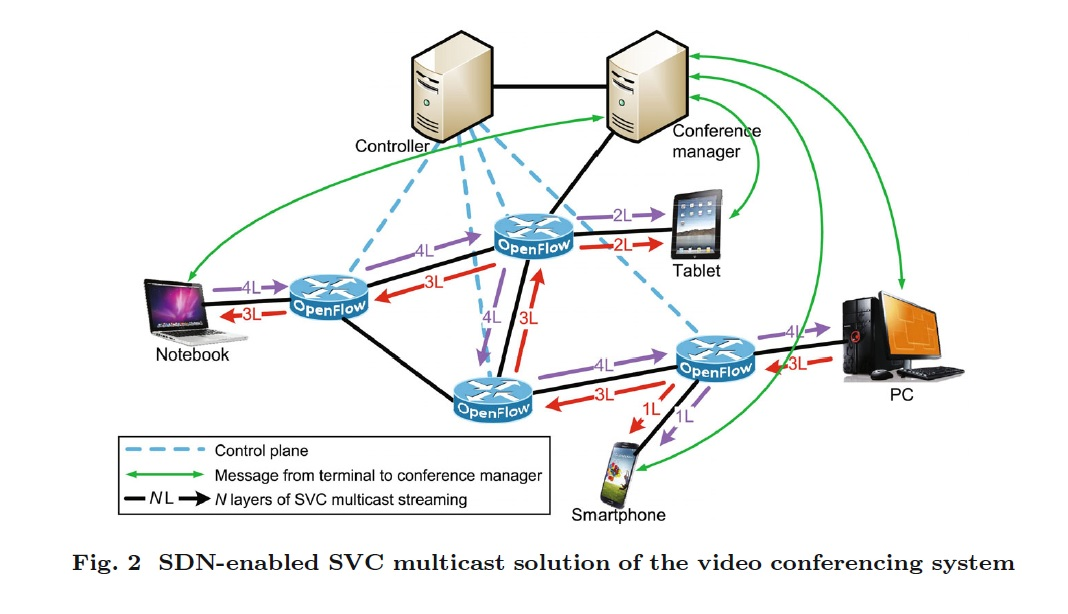
\includegraphics[width=\textwidth]{svc-sdn-video-conf.jpg}

When suffering from network congestion,
the controller is capable of configuring the Open-
Flow switches to dynamically decrease the number of
SVC layers through the corresponding multicast tree
to avoid annoying playback interruptions.

obtain link information between the switch and other connected devices
by a protocol called the link layer discovery protocol (LLDP)

uses ‘statistics’ messages to detect the
congestion event

The experimental results indicated that SDNenabled
SVC multicast works better than the
other solution


\cite{al2018adaptive}
focus on video conferences

The first algorithm sets up the initial multicast
trees for a given call. It optimally places the stream layer adaptation function inside the core network in order
to minimize the bandwidth consumption. This algorithm has two versions: the first one, based on shortest path
trees is minimizing the latency, while the second one, based on spanning trees is minimizing the bandwidth
consumption. The second algorithm adapts the multicast trees according to the network changes occurring during
a call. It does not recompute the trees, but only relocates the stream layer adaptation functions.

Afterward, each receiver is linked to the tree through the
shortest path to any node already in the tree - scale issue

does the paper deal with link failures?
it's mainly focused on wireless links that change bandwidth dynamically, which is a private case of bandwidth changes in the network.

events that may happen in the network and influence the tree topology:
access link variation - SDN controller is aware of bandwidth variations
background traffic - statistics collected from network elements
topology change - link failure, node failure - SDN controller is aware
new subscriber - Video Manager is aware

A participant is, at the same time, a sender of its video
stream and a receiver of video streams from all other participants - true for video conference , not for live video streaming

Participants are considered to be connected wirelessly to their
node by a 4G cellular technology such as LTE

We assume the SVC layers consisting of a base layer L1, and three enhanced
layers L2, L3, and L4. However, our algorithms can be easily generalized
to any number of layers

a given layer can be used only
if all the lower layers are also received.

Each participant accepts the
highest number of layers allowable by its downlink capacity - we offer the user the ability to ask less layers than possible

several participants can be connected to the same
node

All SVC layers belonging to the video stream emitted by one
sender, follow the same paths - not optimal

The SDN controller knows the complete topology of the network,
the position of the participants

The function SortReceivers()(line 4) sorts the
receivers ���� first, from the highest receiving bitrate to the lowest, then
from the closest (to the sender) to the farthest - sort by distance from source is expensive in terms of run time

Steiner tree \cite{winter1987steiner}

We evaluate the different algorithms on random topologies according
to two models:
• Erdős–Rényi model (ER) [42].
• Magoni–Pansiot model (MP) [43]; where the degree distribution
follows a power law (as on the Internet and in large communication
networks). It is based on an algorithm that performs a
sampling on measured Internet maps.

\end{document}
